\chapter{Background}\label{C:background}

A literature research was performed to inform design decision made in this project, and to evaluate any existing research. It will discuss buck converter design factors and topologies, as well as the various different methods of PWM generation. In performing this literature research, we searched Google Scholar, Engineering Village, and Te Waharoa to find designs that utilised variable frequency PWM. 

These searches returned no research relevant to the designs of this project, with the only related work focusing on the electromagnetic noise reduction using randomised frequency modulation \cite{Roman2001,Familiant2016}. Because of this, research was instead performed to inform the design of the buck converter and the generation of PWM signals.

\section{Pulse Width Modulated Signal Generation}\label{S:PWM_back}

Pulse width modulation (PWM) is a digital signal generation technique shown in \Cref{F:PWM}, in which the Period $T$ of the signal is held constant, while the ratio of its logic high period $T_{on}$ to logic low period $T_{off}$ is modulated. This ratio of high period to the low period is referred to as the duty cycle of the PWM signal and is often expressed as a percentage, this can be seen in \Cref{F:Duty}.\\

PWM signals are used in a wide variety of applications for both digital and analogue electronics. PWM is often used to generate analogue signals from digital components by varying the average voltage of the digital PWM signal over time \cite{Tareen2019}. PWM is also used to control the switching elements contained within switch mode power supplies using this same principle, as discussed in \Cref{S:buck_back}. With regard to this project, we will be looking to generate a PWM signal that can be modulated in both duty cycle and frequency.

\begin{figure}[H]
      \centering
      \begin{subfigure}{0.45\textwidth}
          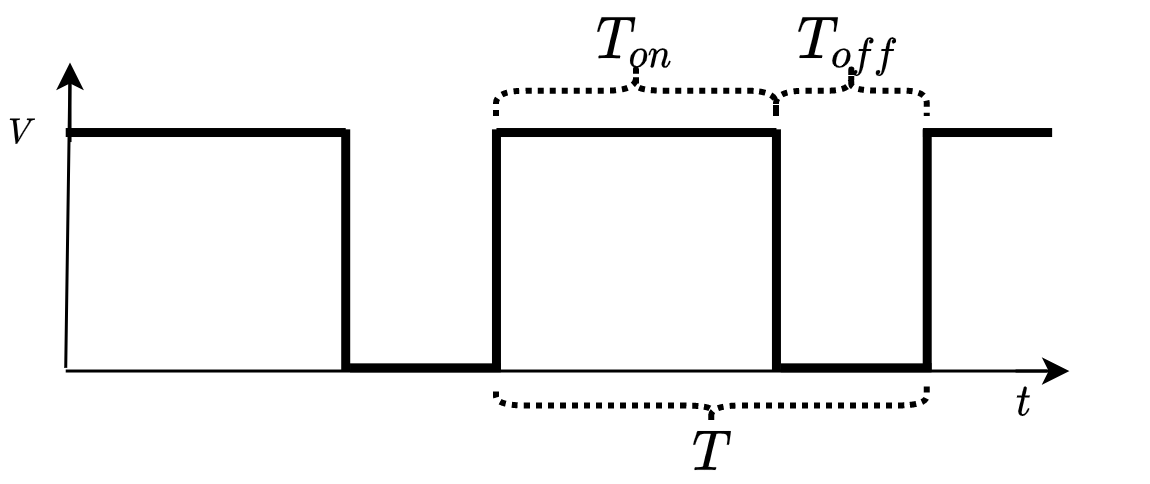
\includegraphics[width=\columnwidth]{background/PWM.png}
          \subcaption{Pulse width modulated signal}
          \label{F:PWM}
      \end{subfigure}
      \hspace{10pt}
      \begin{subfigure}{0.5\textwidth}
          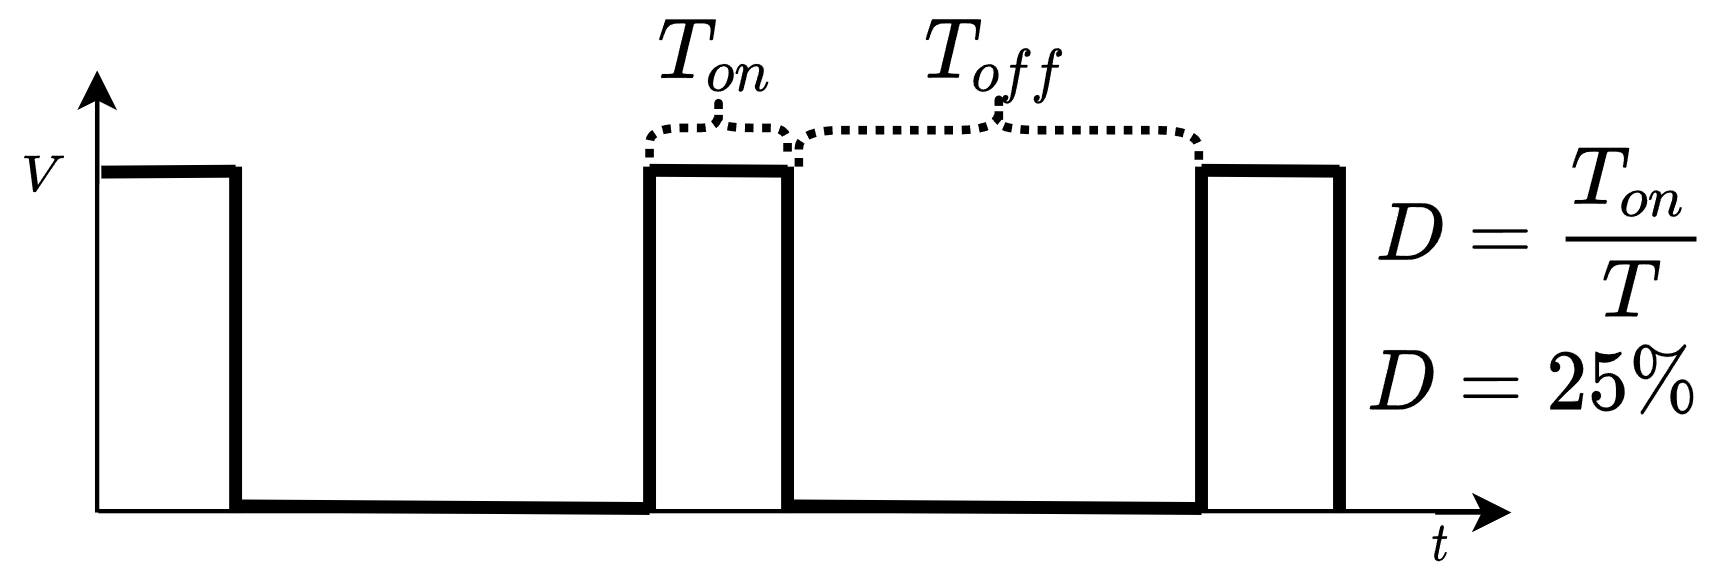
\includegraphics[width=\columnwidth]{background/Duty_cycle.png}
          \vspace{-6pt}
          \subcaption{Duty cycle calculation}
          \label{F:Duty}
      \end{subfigure}
      \caption{Pulse width modulated signal characteristics}
      \label{F:PWM_description}
  \end{figure}

\subsection{Analogue PWM Signal Generation} \label{S:analogue_PWM_back}

Designing a PWM signal generator using analogue components has three distinct stages required to generate the signal. These stages can be seen in \Cref{F:analogue_PWM}, and include clock generation, triangle wave generation, and signal comparator stages \cite{Caldwell2013}.\\ 

The clock generation stage generates a square wave clock signal at a set frequency. This is usually done using a quartz crystal oscillator, or another form of resonating oscillator circuit. The triangle wave generating state must take the clock signal from the previous stage, and produce a triangle wave of the same frequency. This stage is most often done using a standard op-amp integrating circuit with unity gain at the resonating frequency of the clock source. The final signal comparator stage will convert this triangle wave into a PWM signal. Using a comparator, a reference voltage can be applied to the non-inverting input, and then the triangle wave can be applied to the inverting input. This will produce a pulse train with the same frequency as the clock source, where the period of $T_{on}$ and $T_{off}$ is set by the reference voltage. 

\begin{figure}[H]
	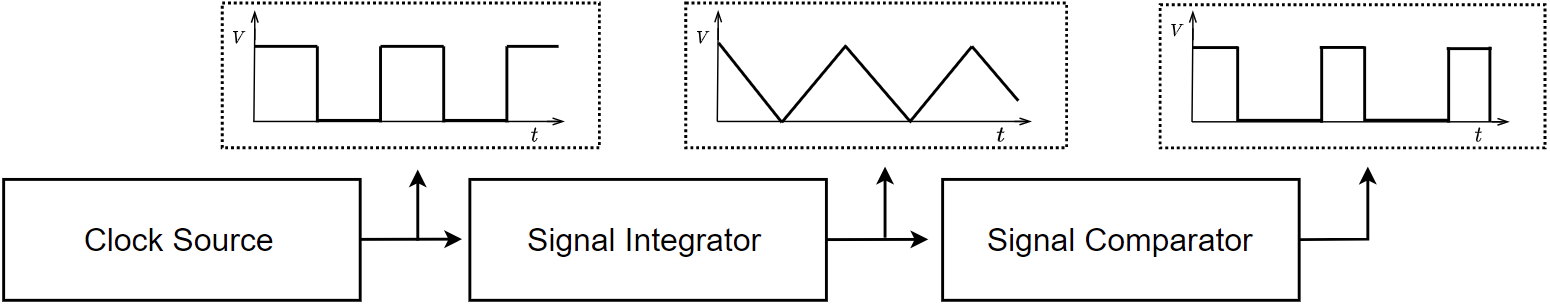
\includegraphics[width = 1\textwidth]{background/Analogue_PWM.png}
	\caption{Stages of analogue PWM generation}
	\label{F:analogue_PWM}
\end{figure}


\subsection{Digital PWM Signal Generation}\label{S:digital_PWM_back}

Designing a PWM signal generator with digital components is far simpler than the method described in \Cref{S:analogue_PWM_back}, and can be done using either a microcontroller or a Field Programmable Gate Array (FPGA). By using an internal timing register that is continually incrementing at a known period we can set a period for our PWM. It is possible to vary the period of the PWM by simply increasing or decreasing the timing registers clock. Next, by toggling a digital I/O when a compare variable is equal to the current value of the timer, we are able to generate a PWM signal with a variable duty cycle \cite{Colley2020}. 
This timing architecture can be simply implemented within an FPGA, but it can also commonly be found within the hardware of most microcontrollers.It should be noted however, that the range of achievable frequencies and duty cycle accuracy will be dependant on an individual microcontrollers clock speed and internal register sizes.

\section{Buck Converters}\label{S:buck_back}

The buck converters is a variant of a switch mode power supply that steps down a DC input voltage to a DC output voltage. They are commonly used in a wide variety of consumer and professional appliances such as laptops, phones, and chargers due to their high efficiency compared to other DC-to-DC step down converters such as linear regulators \cite{Mohan2012}.\\

The basic operational components of a buck converter can be seen below in \Cref{F:buck_func}. From this we see that a buck converter has three main elements, the input voltage source, two switching components, and an output filter across the load. In the case of \Cref{F:buck_func}, the first switching component is an actively controlled switch such as a MOSFET or transistor, and the second a passive switching diode. This configuration of an active and a passive switch is known as the non-synchronous buck converter topology, if the passive diode were to be replaced with a second active switch the topology would be considered synchronous. Although both topologies function under the same fundamental principles, the non-synchronous topology is easier to implement with the drawback of higher losses and therefore lower efficiency.\\

It can also be seen from \Cref{F:buck_func} that a buck converter has two operating states that are controlled through the activation of these switching components. By toggling these switching components at high speed though the use of PWM, we can control the current flowing through the inductor of the output filter. By controlling this current we are also able to directly control the current through, and voltage across the output load of the converter. Using this, buck converters will often have a feedback control system in their design to be able to actively control and regulate the output voltage during usage. This controller will vary the duty cycle of the the switching PWM signal, thereby varying the output voltage of the buck converter as shown in \Cref{E:V_out}.\\

\begin{figure}[H]
	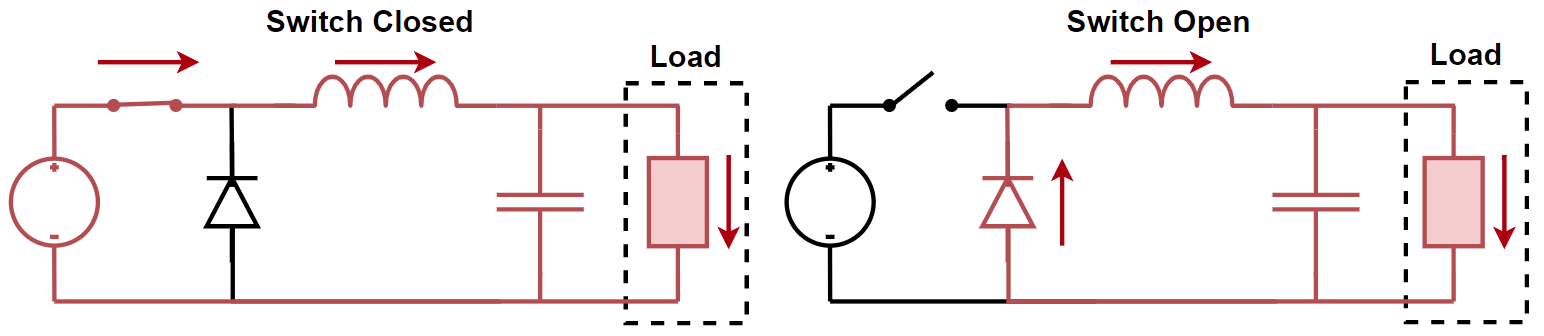
\includegraphics[width = 1\textwidth]{background/Buck_Functionality.png}
	\caption{Operating states of a buck converter}
	\label{F:buck_func}
\end{figure}


\subsection{Buck Converter Design}\label{S:buck_design_back}

The design of a common buck converter has two primary considerations, the output voltage of the converter $V_0$, and the inductor current ripple of the converter $\Delta i_L$. These considerations can be specified by designing the buck converter using \Cref{E:V_out} \& \Cref{E:delta_i} \cite{Mohan2012_Design,Hauke2015}.\\ 

When designing a buck converter the first design specification that must be met is the output voltage. In \Cref{E:V_out} the output voltage can be directly related to the input voltage $V_{in}$ and the switching duty cycle $D$. Using this equation it is possible to directly set the output voltage of the buck converter by varying this duty cycle.

\begin{align}\label{E:V_out}
	V_o &= D \cdot V_{in}
\end{align}

Once the output voltage has been specified, the inductor current ripple can be calculated and specified with \Cref{E:delta_i}. This equation allows for the inductor current ripple to be directly related to the inductor size $L$, and the PWM switching frequency $f_s$. This allows the the specification of the inductor current ripple through the varying of these two values.

\begin{align}\label{E:delta_i}
   \Delta i_L &= \frac{ V_{o} \cdot \left( 1 - D \right) } {L \cdot f_s}
\end{align}

These two equations will be used to inform the designs and specifications of this project, and will be discussed in detail in \Cref{S:specs_design}.




\section{Current Sensing}\label{S:current_sense_back}

Current sensors are transducers that converter an input current to an easily measured output voltage that is proportional to the current through the sensor. Current sensors operate on one of two principles, Ohm's law, Faraday’s and Ampere’s law \cite{current_sensor_types}.  Ohm's law describes how when current flows through a resistive element a voltage drop will occur. Sensors operating under this principle will measure the voltage drop across a known resistance, and are referred too as direct sensors as they directly effect the circuit. Faraday’s and Ampere’s law describes how a changing electric flux will induce a changing magnetic field, and a changing magnetic field will induce a changing magnetic flux. Sensors operating under this principle will use the magnetic field induced by the current through the sensor to produce a voltage proportional to that current, and are referred to as indirect sensors as they make no direct contact with the circuit being sensed. 


\subsection{Current Sense Amplification}\label{S:current_shunt_back}

Current sense voltage amplification sensors are a form of direct sensor, working on the principle of Ohm's law $I=\frac{V}{R}$. By sensing the voltage dropped across a known value resistive element (Often called the current shunt), it is possible to calculate the current that is flowing through the element. This form of current sensing is very simple to implement in theory, however it has the effect of altering the system being sensed by adding a resistive load, and thereby increasing the losses of the system. 

To mitigate the effects of this sensing on a circuit, a smaller resistive load can be used. However, this will also decrease the measurable voltage across the load, and therefore decrease the precision of a taken measurement. Because of this, shunt based current sensors are often paired with an operational amplifier of known gain. This combination allows for accurate amplification of the shunts voltage drop, increasing the precision of measurements, and allowing for drastically smaller shunt resistors. 


\subsection{Hall Effect Sensors}\label{S:hall_effect_back}

brief overview of hall effect sensors. They function by measuring the magnetic flux density, meaning that they are commonly used to sense the presence of a magnet. However since a current flowing though a wire will produce a magnetic flux, they can also be used to measure current flow.

Because of this operation, they are able to sense a current without contacting or altering the circuit. This means that they are commonly used in the measurement of high voltage or high current circuits, as they will remain completely isolated from the circuit being sensed, and will also not dissipate power from the sensed circuit. This provides large safety advantages, and can often decrease the complexity of the sensing circuit. 

Hall affect sensors do however suffer from a lack of precision. Due to their operation, their measurements will constantly be offset by any ambient magnetic flux. This means that they are not commonly used for the sensing of small signal currents, as the noise floor of the Earth's own magnetic field can often be larger than the signal being sensed.  






\section{Control Systems}\label{S:control_back}

Discuss the basics of control theory, and how a controller can be implemented on a digital system within discrete time. 

\begin{itemize}

    \item
        Discuss in very general terms what a control system is what what it seeks to do in a system.

    \item
        Discuss what the control system will be doing in the case of this project. Talk about how a controller will be used to control both the output voltage of the converter, and the inductor ripple of the converter.

    \item 
        Discuss the design, use, and implementation of a PID controller within a system. 

\end{itemize}

\subsection{PID Controllers}\label{S:PID_back}